\section{Mesh generation}

\subsection{blockMesh}
\paragraph{}The definition of the \textit{blockMeshDict} is the first part that needs to be defined in order to simulate the case. 
Only the first two stages of the turbofan engine will be simulated, so we have to make sure that the \textit{blockMesh} includes them.
\paragraph{}The domain of the mesh is a $0.58$x$2.3$x$2.3m$ rectangular prism and the vertices are as follows:\\
\texttt{\small{vertices\\*
(\\*
    (0.77 0   0)\\*
    (1.35 0   0)\\*
    (1.35 2.3 0)\\*
    (0.77 2.3 0)\\*
    (0.77 0   2.3)\\*
    (1.35 0   2.3)\\*
    (1.35 2.3 2.3)\\*
    (0.77 2.3 2.3)\\*
)
	}
}

\paragraph{}Once the boundaries of the \textit{blockMesh} are defined, the number of cells that it will have has to be set. It has to be taken into account that a very dense mesh will not be efficient when simulating the case. On the other hand, a very coarse mesh will not be efficient either because additional divisions will have to be set when generating the refined mesh with \textit{snappyHexMesh}. Thus, a compromise solution between a mesh with a very high number of cells and a very low number of cells has to be attained.

\paragraph{}This basic mesh has been divided every $0.05m$. It means that we have done 12 divisions in the x direction, 46 on the y direction and 46 more on the z direction. Obviously, the vertex numeration has been kept the same as the one that comes as default in every tutorial case; so, it was easier to define the inlet face of the \textit{blockMesh} as well as the outlet face that will be used to define the boundary conditions.

\begin{footnotesize}

\begin{verbatim}
  
/*--------------------------------*- C++ -*----------------------------------*\
| =========                 |                                                 |
| \\      /  F ield         | OpenFOAM: The Open Source CFD Toolbox           |
|  \\    /   O peration     | Version:  4.0                                   |
|   \\  /    A nd           | Web:      www.OpenFOAM.org                      |
|    \\/     M anipulation  |                                                 |
\*---------------------------------------------------------------------------*/
FoamFile
{
    version     2.0;
    format      ascii;
    class       dictionary;
    object      blockMeshDict;
}

// * * * * * * * * * * * * * * * * * * * * * * * * * * * * * * * * * * * * * //

convertToMeters 1;

vertices
(
    (0.77 0   0)
    (1.35 0   0)
    (1.35 2.3 0)
    (0.77 2.3 0)
    (0.77 0   2.3)
    (1.35 0   2.3)
    (1.35 2.3 2.3)
    (0.77 2.3 2.3)
);

blocks
(
    hex (0 1 2 3 4 5 6 7) (12 46 46) simpleGrading (1 1 1)
);

edges
(
);

boundary
(
    frontAndBack
    {
        type patch;
        faces
        (
            (3 7 6 2)
            (1 5 4 0)
            (0 3 2 1)
            (4 5 6 7)
        );
    }
    inlet
    {
        type patch;
        faces
        (
            (0 4 7 3)
        );
    }
    outlet
    {
        type patch;
        faces
        (
            (2 6 5 1)
        );
    }
);

// ************************************************************************* //

\end{verbatim}

\end{footnotesize}

\paragraph{}The log obtained when the mesh has been generated is as follows:

\texttt{\\*
Writing polyMesh\\*
----------------\\*
Mesh Information\\*
----------------\\*
  boundingBox: (0.77 0 0) (1.35 2.3 2.3)\\*
  nPoints: 28717\\*
  nCells: 25392\\*
  nFaces: 79396\\*
  nInternalFaces: 72956\\*
----------------\\*
Patches\\*
----------------\\*
  patch 0 (start: 72956 size: 2208) name: frontAndBack\\*
  patch 1 (start: 75164 size: 2116) name: inlet\\*
  patch 2 (start: 77280 size: 2116) name: outlet\\
  \\
  End
}

\begin{figure}[h!]
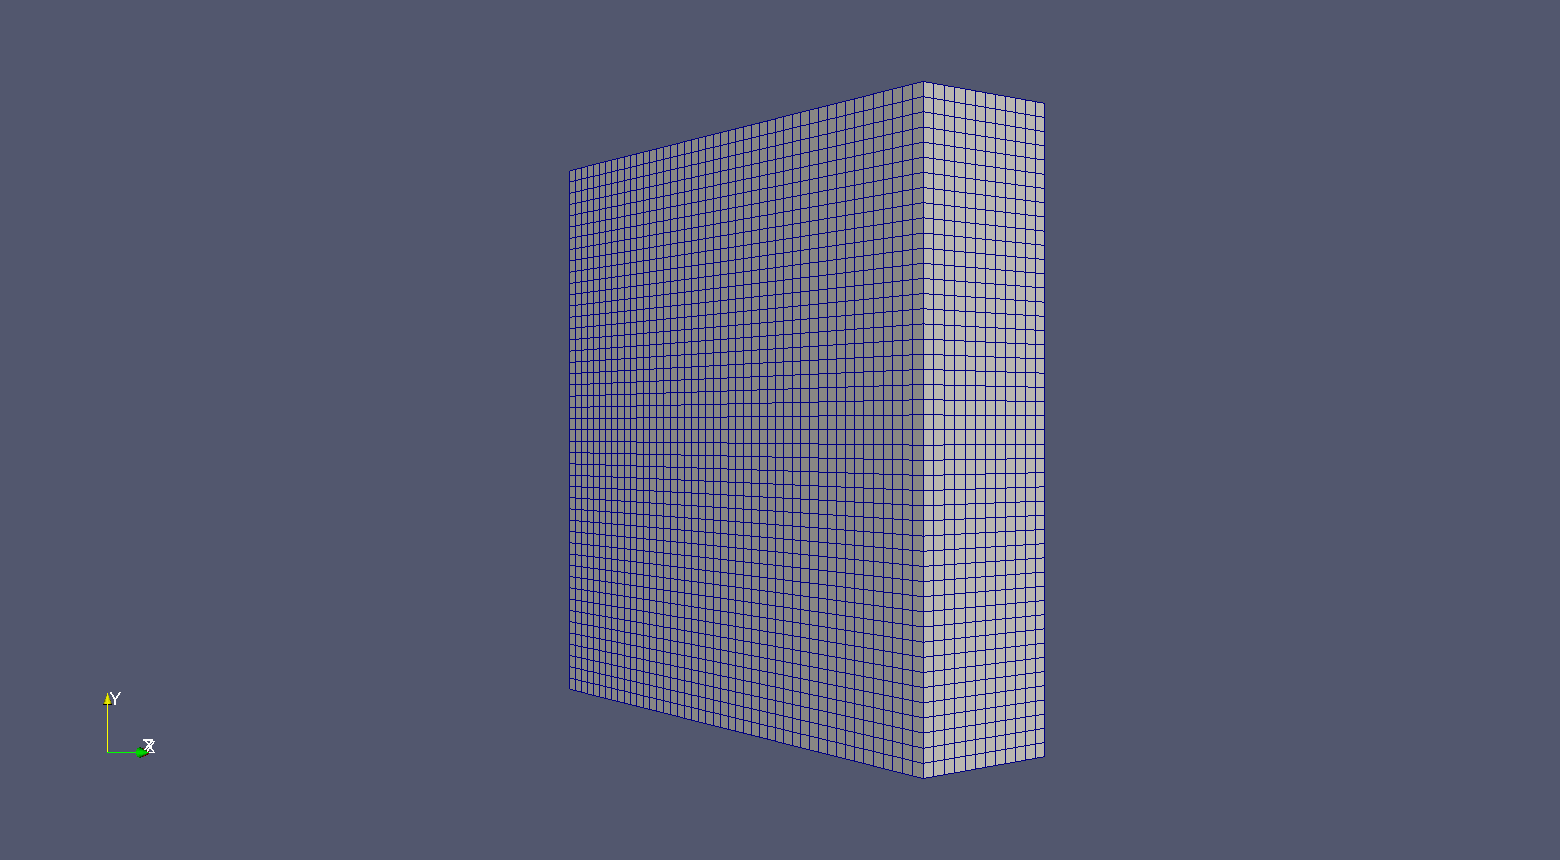
\includegraphics[scale=0.26]{./mesh/screenshots/blockmesh}
\centering
\caption{blockMesh}
\end{figure}

\subsection{Mesh refinement}

\paragraph{}To refine the mesh, the \textit{snappyHexMesh} utility, included in OpenFoam, which is used and several parameters have to be modified in order to obtain a dense mesh that is suitable for the simulation of this complex geometry. Additionally, it has to be considered that a particular geometry is has a relative velocity; this is, the rotor is rotating, and so the first and second stages of the Low Pressure Compressor of the turbofan engine, while the nacelle and the combustor are static. 

\paragraph{}\textbf{FALTA EXPLICAR SURFACE EXTRACT}

\paragraph{}A comparison between the coarse mesh and the refined mesh generated is presented below.

\subsubsection{Coarse mesh}
\paragraph{}The number of control volumes in the mesh is 40.

\begin{figure}[h!]
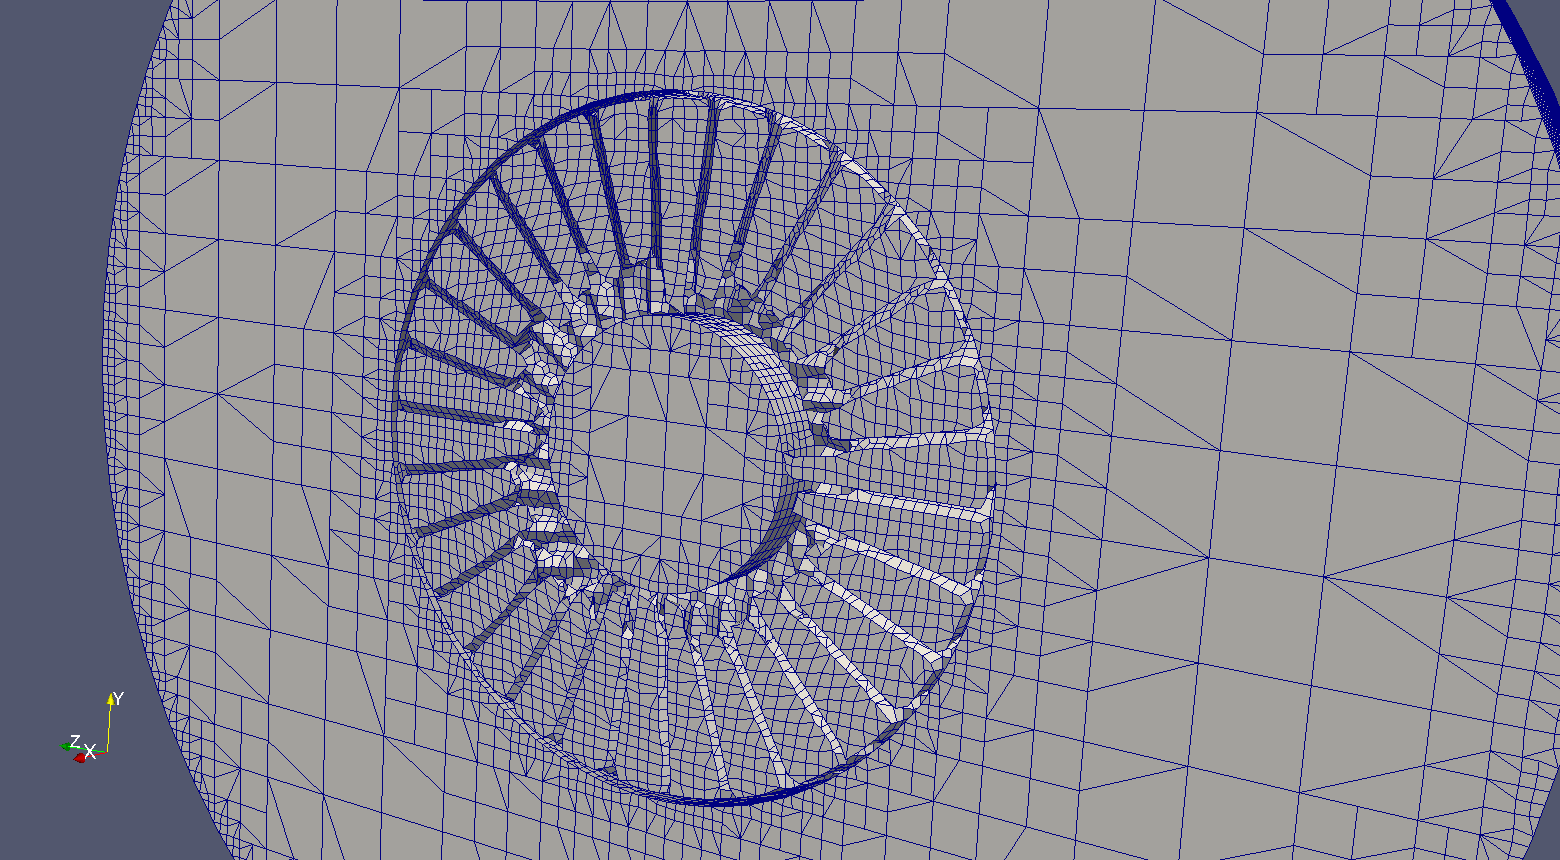
\includegraphics[scale=0.26]{./mesh/screenshots/coarse2}
\centering
\caption{Detail of the coarse mesh}
\end{figure}

\begin{figure}[h!]
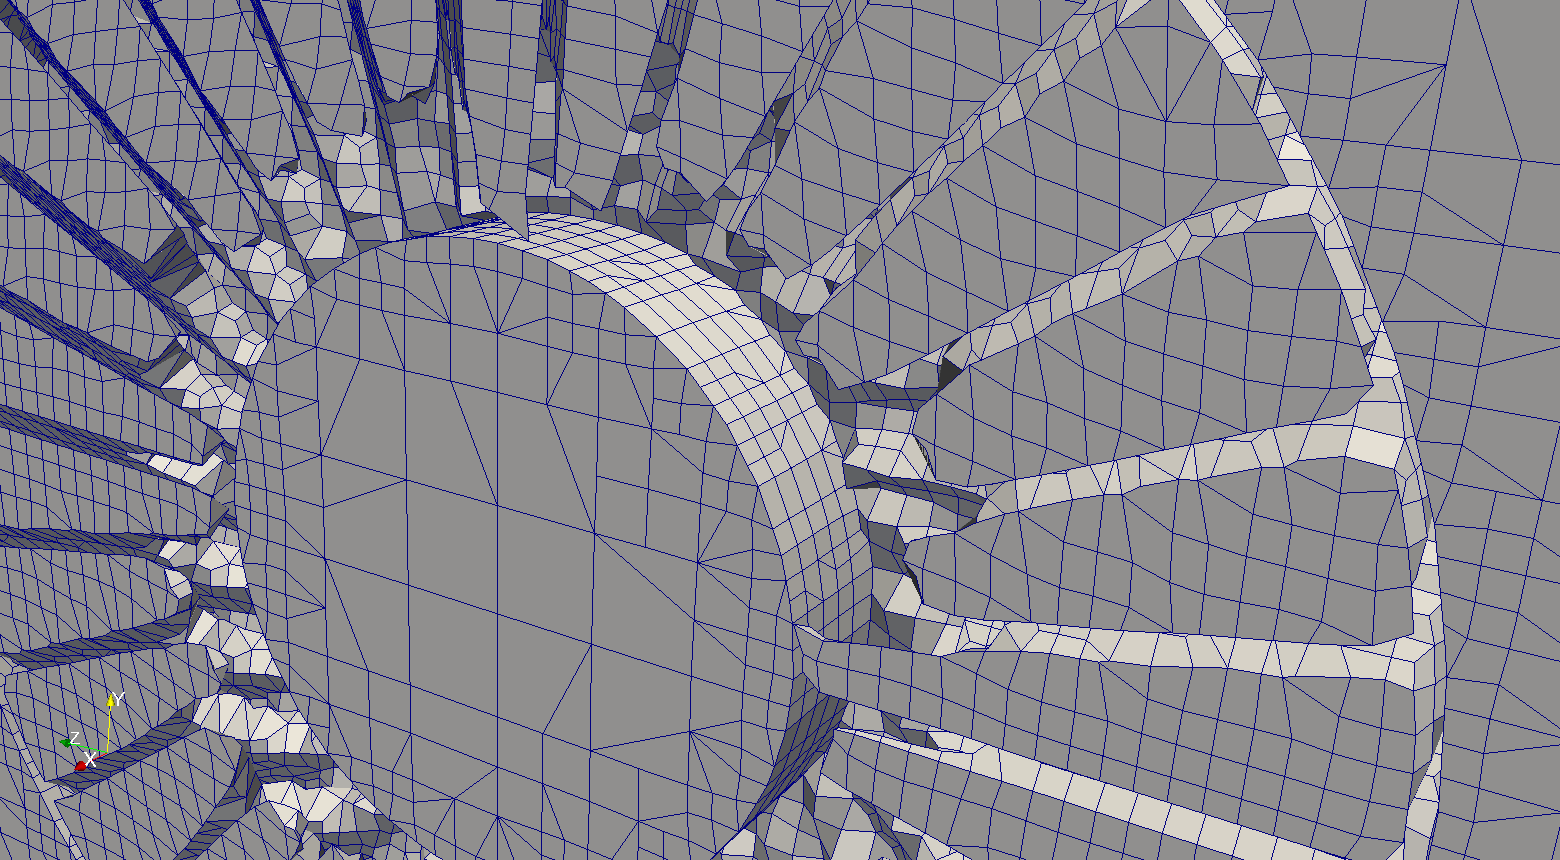
\includegraphics[scale=0.26]{./mesh/screenshots/coarse3}
\centering
\caption{Detail of the coarse mesh}
\end{figure}

\subsubsection{Standard mesh}

\begin{figure}[h!]
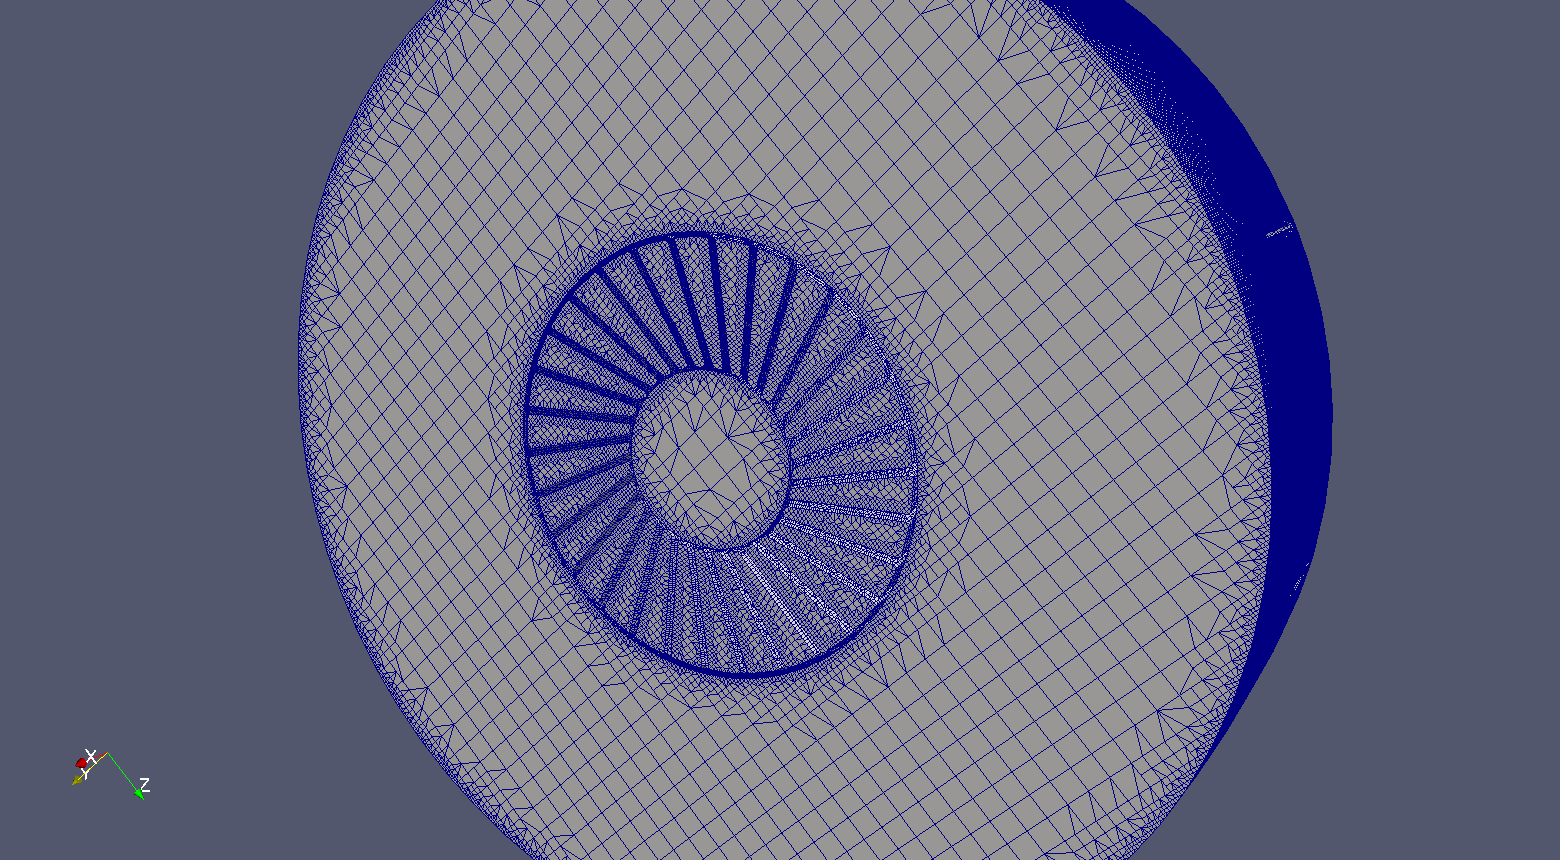
\includegraphics[scale=0.26]{./mesh/screenshots/std2}
\centering
\caption{Detail of the standard mesh}
\end{figure}

\begin{figure}[h!]
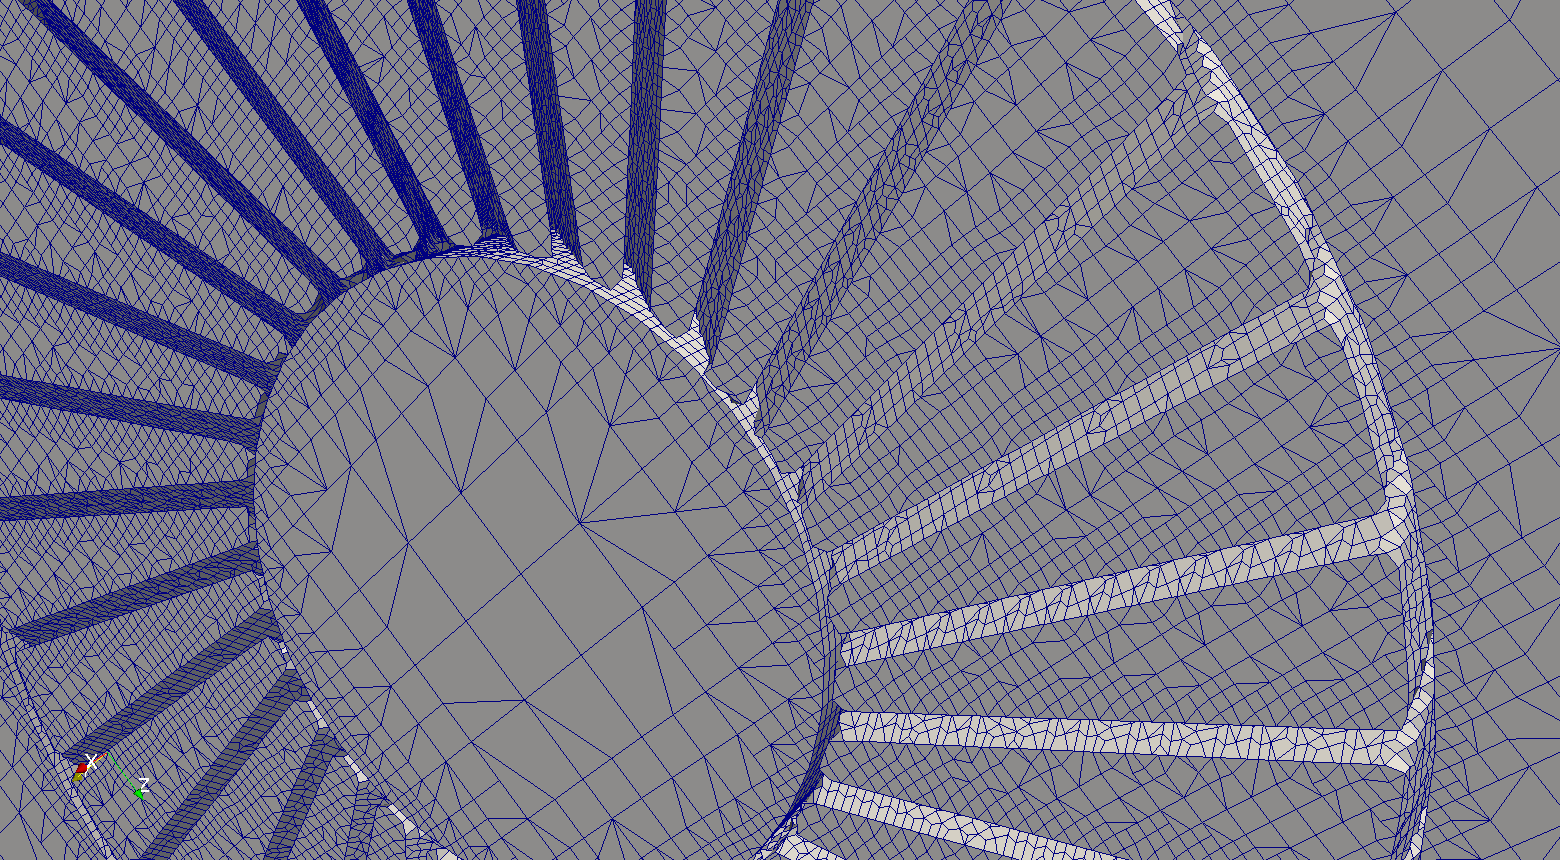
\includegraphics[scale=0.26]{./mesh/screenshots/std3}
\centering
\caption{Detail of the standard mesh}
\end{figure}

\subsubsection{Dense mesh}

\begin{figure}[h!]
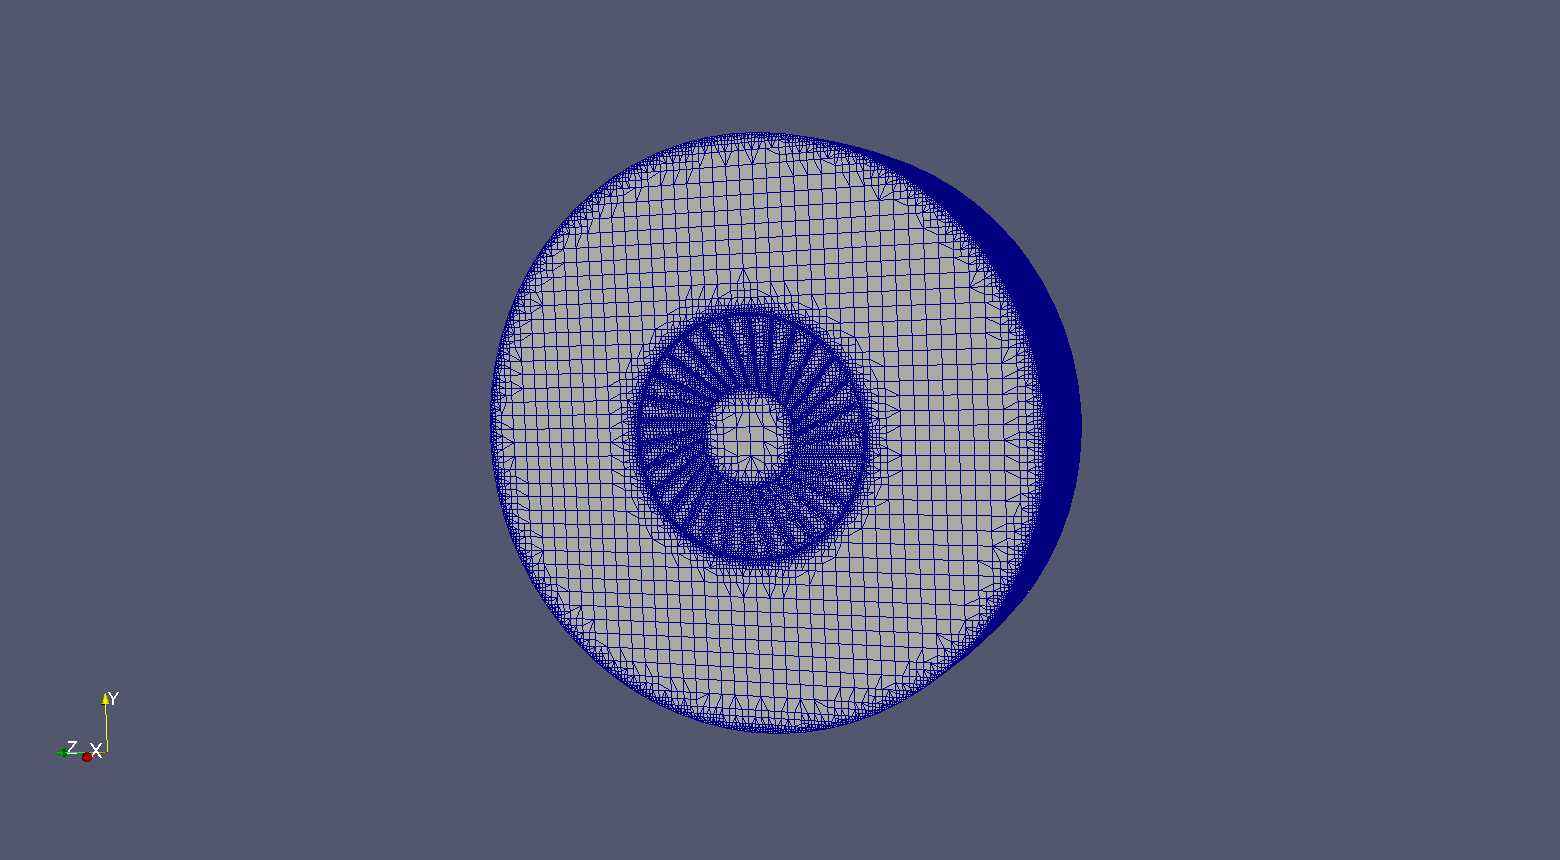
\includegraphics[scale=0.26]{./mesh/screenshots/Xtreme1}
\centering
\caption{Detail of the coarse mesh}
\end{figure}

\begin{figure}[h!]
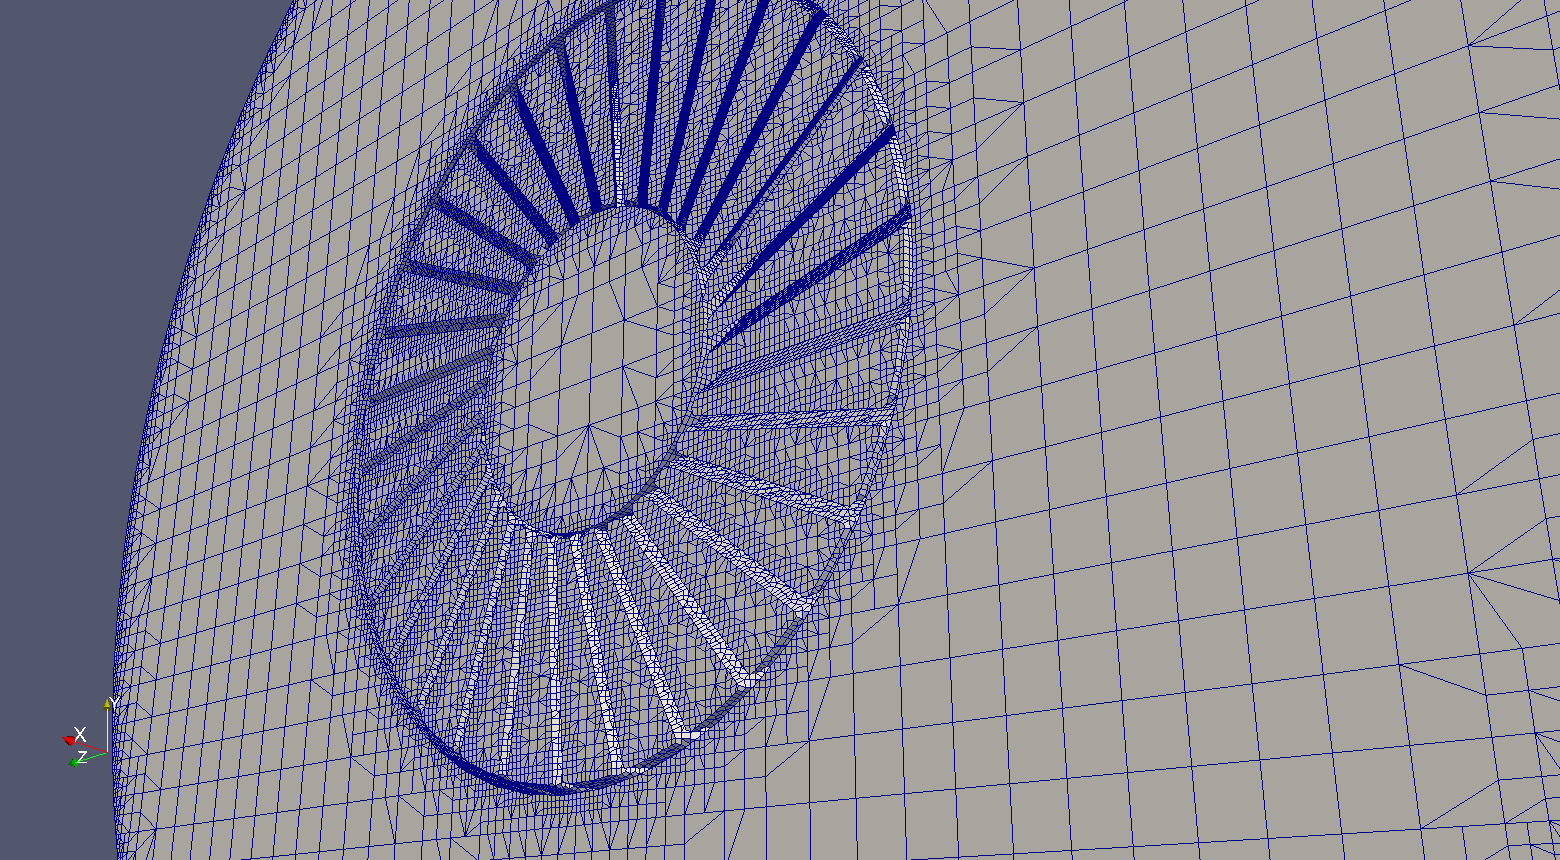
\includegraphics[scale=0.26]{./mesh/screenshots/Xtreme3}
\centering
\caption{Detail of the dense mesh}
\end{figure}

\begin{figure}[h!]
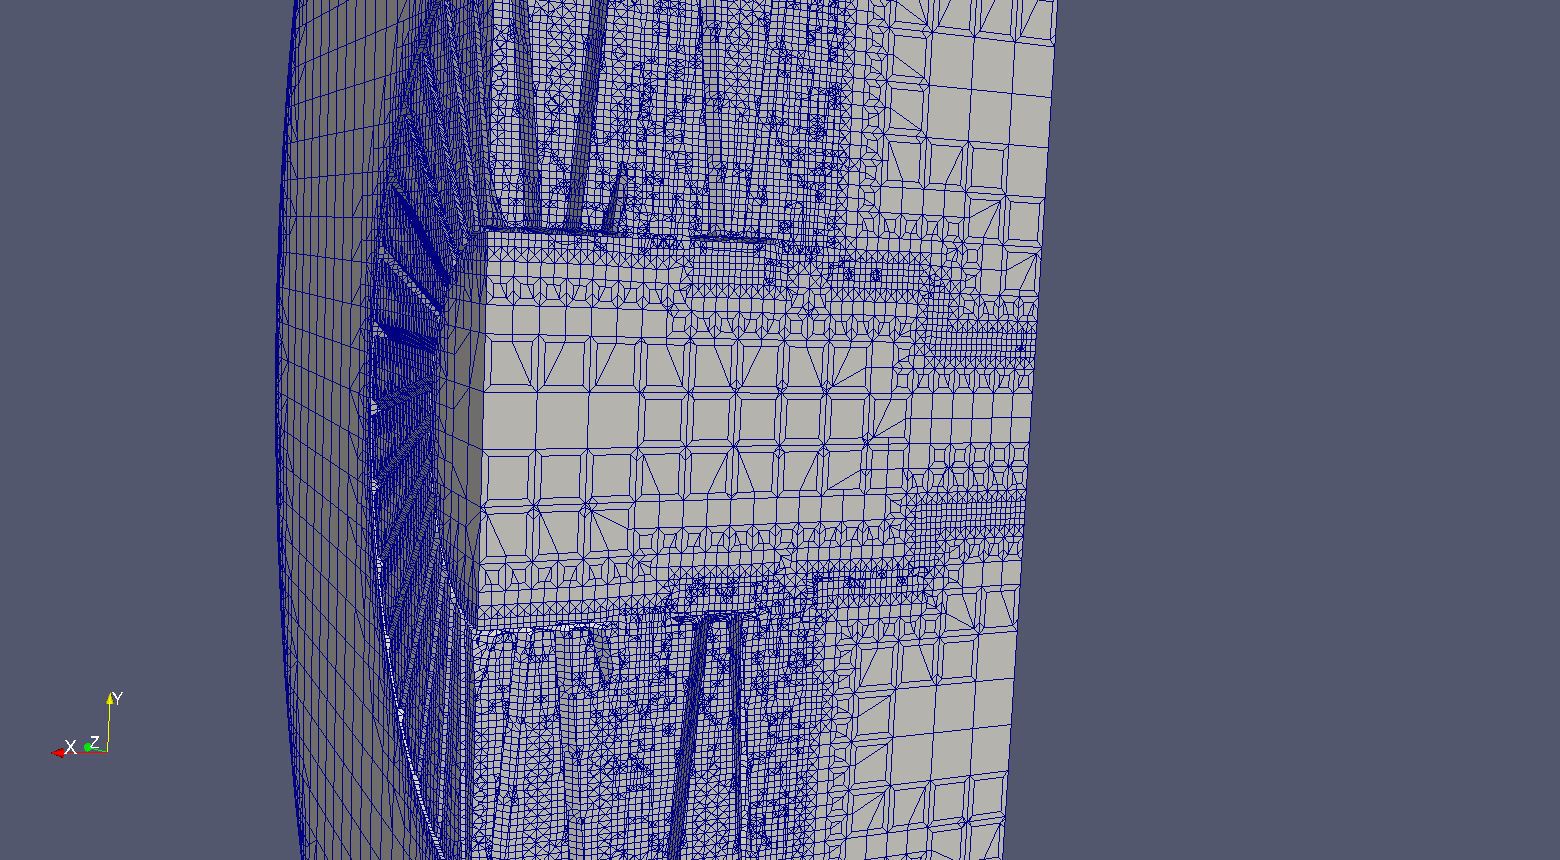
\includegraphics[scale=0.26]{./mesh/screenshots/Xtreme5}
\centering
\caption{Detail of the dense mesh}
\end{figure}
